\chapter{Evaluation of IP/TCP/UDP options over public networks}

As the Internet evolves, so do the expectations for new network protocols. Whether said protocols pertain to traffic encryption, packet source authentication or routing optimization, all are faced with the same initial hurdle: the uncertainty of their compliance with the myriad filtering policies employed by virtually just as many middleboxes. This incertitude has only been exacerbated by the continual ossification of the foundational internet protocols. An immediately apparent indicator of this suggested entrenchment is the maladroit adoption of new standards and acceptance of implementations conforming to well-established specifications. We draw attention to RFC 7126, offering recommendations on filtering packets with IPv4 options due to widespread misuse. Its necessity after upwards of thirty years since this IP extension mechanism was provisioned in RFC 791 is epitomic of the issue at hand. Regardless of the underlying causes that lead to this predicament, the objective is not necessarily to remedy but to circumvent the obstacle that it poses.

In this chapter we try to address both of the aforementioned problems. In reponse to the former proposition, we perform an investigation of protocol options acceptance in the Internet and establish their viability as conduits for the purpose of packet tagging. The latter of the two problems we address by means of a state of the art survey. This survey is meant to inform the reader on the challenges of emplying automated testing for establishing trust in non-deterministic builds of network applications.

\section{Problem statement}

In this chapter, we try to address the issue of protocol ossification. As such,
we perform an investigation of protocol options acceptance in the Internet and
establish their viability as conduits for the purpose of packet tagging. To this
end, we propose the following research questions:

\textbf{RQ1: Is the current state of affairs in the wider Internet adequate for already standardized protocol options?}
Extant protocols had been designed under the assumption that the existing fixed-length headers would at some point become insufficient for encapsulating the information needed by supplementary mechanisms. Consequently, most of them included a variable-length options feature allowing their incorporation as the need arises. The benefits are most evident when observing how TCP is reinforced by the Window Scaling option (increases the maximum window size from 64Kb to 1Gb) or the Selective Acknowledgement option (allows specifying a finite range of lost packets). In their absence, TCP would cease to be viable in high-latency, high-bandwidth environments such as WANs. While options were initially overlooked in lieu of redefining existing fields to better fit specific purposes of certain users, the approach has been thoroughly discouraged by the open standards organizations and the community at large. Despite the growing demand for extending current protocols, Autonomous Systems (AS) proved resistant to this change. Although some options have been standardized, their acceptance remains highly dependant on middlebox manufacturers.

\textbf{RQ2: Can new protocol options be attached to a packet without compromising its conformity to the filtering schemes?}
When the aforementioned protocol extension systems were first defined, a number of option identifiers (i.e.: codepoints, kinds) were designated to features immediately necessary at the time (e.g.: the IP Security option or the UDP Authentication and Encryption option). In order to properly administer the growing number of independent projects and prevent the unauthorized usage of unassigned codepoints from becoming praxis, IANA had reserved certain ranges for this purpose. This, in turn, lead to the introduction of experimental IDs as a method of sharing the yet limited assigned ranges, when testing in common environments. Nonetheless, there have been known cases of unpermitted use of certain codepoints, some overlapping with established options (e.g.: TCP User Timeout). Seeing how these unregistered and experimental options are practically unknown to most middleboxes, an understandable concern is whether they will be accepted without any further verification or simply dropped.

\textbf{RQ3: Does the annotation scheme under consideration interfere with the base functionality of any protocol or application?}
Assuming that a modified packet is able to traverse the network unthwarted, the need to ensure normal operation of applications whose traffic falls within the purview of the scheme under test is paramount. Ideally, the packet alteration is handled outside the scope of the application itself, either in kernel (e.g.: DCCP's Explicit Congestion Notification) or by deference to another userspace process (e.g.: tcpcrypt's packet manipulation using NetfilterQueue). However, this is not always the case. Employing kernel bypasses can be rightfully motivated by practical limitations, such as IRQ storms during DDoS attacks (most CPU time is used to receive packets, not process them). During such attacks, \texttt{iptables} reaches a state of saturation at approximately 1M packets per second (pps). While solutions based on eBPF are known to be able to drop up to 15Mpps and quickly recover from a state of FIFO tail dropping, the technology is still new and imposes stringent constraints on the developer. Meanwhile, solutions based on frameworks such as Intel DPDK or PF\_RING are more likely to be incompatible with any new annotation scheme. Consequently, a large-scale testing environment is required to validate any new addition to well-established protocols.

We claim the following contributions:
\begin{itemize}
    \item We offer a tool\footnote{Code available at \url{https://github.com/RaduMantu/ops-inject}} capable of intercepting specific packets and annotating them with user specified, per-protocol option types. The options are generated in their entirety by a decoder that allows for easy integration of new option types, as well as protocols.
    \item We propose a framework for assessing an annotation system's compliance with firewall policies and provide configuration scripts and templates for cloud experimentation under the primary available providers (i.e.: Google Cloud, AWS, Microsoft Azure, Digital Ocean).
    \item We evaluate current Layer 3 and Layer 4 protocol extension mechanisms and deliberate their suitability as a basis for developing new extensions.
\end{itemize}

\section{Architecture}

\subsection{Annotation tool}

In testing different features of Layer 3 and Layer 4 protocols, a usual approach consists of generating synthetic traffic and bypassing the network stack of the originating host. We decided to forgo this method in favor of a more practical alternative: modifying real traffic. The primary advantage of the latter scheme over the former is the ability to verify not only that the annotated packets can be successfully transmitted over the network, but also that their alteration does not impact higher level protocols in the OSI stack. Additionally, the flexibility in assessing compliance with stateful firewalls alleviates the effort that would have otherwise been required to simulate sufficiently credible sessions.

These aspects gave impetus to the development of a method to insert multiple protocol specific options in outgoing traffic. One of the essential characteristics of the resulting tool is the capacity to easily implement new options for existing protocols or to register new protocols altogether. Limited by the extent of our needs for this experiment, session tracking falls outside its purview. As a result, options such as MultiPath TCP are not available for testing. Instead, all options should either be static in nature (e.g., NOP) or depend entirely on the information available in a single packet's header and payload (e.g., alternative checksums). Otherwise, its use may be limited to determining only whether the initial packet was able to traverse the network (e.g., TCP timestamps).

Next, we present a summary overview of the tool's operation. Initially, the user adds one or more \texttt{iptables} rules with an \texttt{NFQUEUE} target. All packets that match one of these rules are redirected into userspace for our tool to evaluate and modify as it sees fit. During the initial invocation of the tool, the user may specify a sequence of bytes that represent option codepoints. For each packet, the codepoints will be expanded to actual TLV entries and inserted into a (potentially new) options section. The NetfilterQueue callback that fulfils this purpose takes three steps towards successful annotation. Next, we describe these steps in greater depth:

\textbf{Options Decoding:} Having access to the packet, as provided by the Netfilter kernel hook, the first step is generating the contents of the options section for a pre-established protocol (i.e., IP, TCP, UDP). Using the user-specified sequence of \texttt{option-type} octets, specific decoder functions are called upon to expand them, thus populating the options buffer. This expansion phase is by and large an arbitrary process. For example, an IP Timestamp Option (\texttt{0x44}) will be translated to a 12 octet buffer containing a single timestamp associated to the source IP address. The generated flags will denote pre-specified address fields as to discourage addition of new timestamps from compliant middleboxes. This inhibition of user agency is a conscious decision intended to simplify the tool's usage. Nonetheless, the decoder functions can be easily modified on a case-by-case basis to accept more information and conform to finer-grained requirements. Note that the options will appear in the order in which they were initially specified by the user. However, the order in which they are generated may vary. For example, a UDP Options Checksum (\texttt{0x02}) is supposed to be placed as close to the beginning of the section as possible, while at the same time requiring all other options to have already been calculated. Consequently, it's decoding is delayed based on a discretionary option priority assignment.

\textbf{Packet Reassembly:} This step modifies the initial packet in order to include the newly generated options. Any related fields (e.g., \texttt{IP.total\_length}) with the exception of the checksum are adjusted to account for the payload offset. Based on user preference, existing options can either be completely replaced, or preserved. In our tests, we employed the former approach in order to exert full control over the content of the options section. Alternatively, existing options would take precedence. In turn, this could lead to overflowing user-specified options to be discarded due to space constraints.

\textbf{Checksum Recalculation:} The reason why this step is separate from the previous is that changes made to a header corresponding to a lower layer can impact the checksum of a higher layer protocol. For example, while IP options are intended to extend only the IP header, the total packet length increases nonetheless. As a result, TCP's or UDP's pseudo-header changes and the Layer 4 checksum does so along with it.

An advantage of relying on the Netfilter framework is that it integrates well with \texttt{ip-xfrm} (kernel-side module that implements the IPsec protocol suite). Usually, VPN implementations are split across both userspace and kernelspace. The former carries out the negotiation required as per the IKE protocol, which establishes up to four Security Associations (SA) and creates a Security Policy (SP). The latter utilizes the SAs for packet encapsulation and encryption but more importantly, it uses the SP to determine which packets are to be passed to the IPsec stack. This decision is taken by consulting an SP database after the packet has traversed the \texttt{OUTPUT} and \texttt{POSTROUTING} chains. If appropriate, the packet is modified and reinserted prior to entering the \texttt{OUTPUT} chain. The \texttt{iptables} rule that identifies the packets which require annotations must be well-defined. Otherwise, the user risks modifying a packet that is protected by the ESP protocol. We consider this approach preferable to excluding packets containing ESP headers. Due to the potential usage of NAT-traversal encapsulation, it would be inefficient to identify the presence of the ESP header. Moreover, allowing UDP packets with destination port 4500 to pass may exempt IKE configuration packets from annotation, contrary to the user's intention.

\subsection{Testing framework}

Irrespective of the type of protocol that may benefit from these extensions, they will in all likelihood be required to interact with cloud-hosted solutions. As a result, we focus our efforts on verifying if and how cloud providers allow the passage of annotated packets through their networks. To this end, we perform a series of inter-regional tests. The structure of the testing environment can be seen in Fig. \ref{extend:ops:fig:architecture}. Initially, the management instance (i.e., localhost) will install the annotation tool, as well as any traffic generation tools under test on each virtual machine. Additionally it will also start \texttt{tcpdump} processes and insert specific \texttt{iptables} rules with the purpose capturing relevant traffic for annotation and later analysis. When testing a certain instance (e.g., the one in me-south-1 region in AWS), a server will be started (1) by issuing a command over a ssh channel. Immediately after, all other instances will be issued similar commands, to start a client (2) and send requests to the server. The resulting traffic will be annotated in both directions. After all communication (3) will have ceased, another instance will be selected as the server. Finally, all \texttt{tcpdump} processes will be killed and the generated packet captures as well as any logs will be downloaded for analysis.

\begin{figure}[htb]
    \centering
    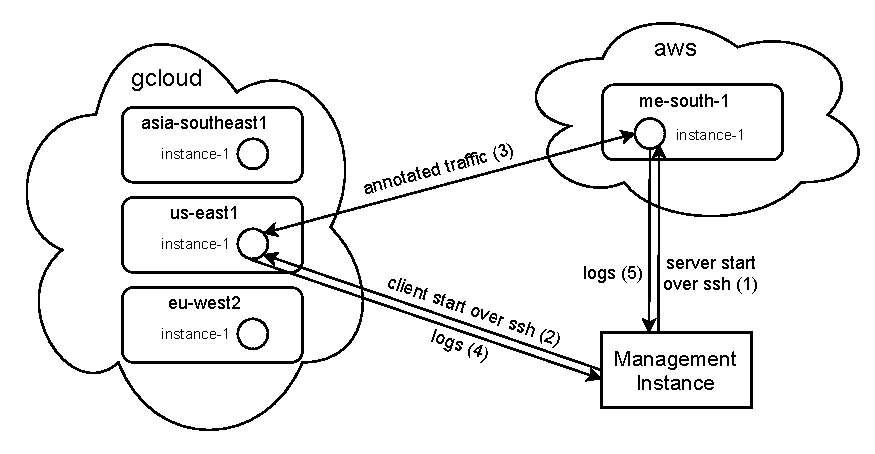
\includegraphics[width=0.8 \textwidth,keepaspectratio]{figures/architecture.pdf}
    \caption{Architecture of the cloud testing framework.}
    \label{extend:ops:fig:architecture}
\end{figure}

The framework is comprised mostly of bash scripts using each provider's CLI management tool. A minimal setup is required: configuring default projects and public keys, enabling billing, and relaxing the firewall rules of their private networks to the extent that they are permitted. The scripts can be classified as management scripts, experiment scripts or analysis scripts, depending on their purpose. Management scripts allow the automatic creation or deletion of VM instances in accordance with a pre-specified list of regions. This list can be freely modified in accordance with the available selection of each cloud provider. Additionally, they administer the configuration of VPNs or that of the annotation tool. Experiment scripts install missing dependencies and generate traffic between any two instances. The commands executed on remote machines are issued over a secure SSH channel. All relevant inbound and outbound traffic is recorded on each instance and eventually imported on the managing host. Any analysis of packet reception and option removal or alteration can be done offline. To this end, we offer a subset of the analysis scripts that we employed in interpreting the network captures, along with samples of said captures. We include only general-purpose scripts that, for example, report overall instance reachability or retrieve AS numbers and names of recorded IP addresses.

Note that this framework is not specifically aimed at evaluating cloud providers. Their preponderance in our tests was meant to verify the compliance to the protocol extension standards in the wider Internet. Given that the credentials are correctly configured on all machines, the experiments can be executed with either a statically defined set of public and private IPs, or via a user-provided means of dynamically generating said set.

